%!TEX root = ../main.tex

\section{Interesting Internal Functions}
\label{section:internal_functions}

MobilityDB is an extension to PostgreSQL and is thus exposed to the user using SQL types and functions, with a large portion of these functions being described in Section \ref{section:general_functions}. Multiple internal functions were necessary to implement these SQL functions, and a few of them are worth mentioning here, due to their particularity and/or difficulty.

\subsection{Rotating Bounding Boxes}
\label{section:bbox}

One implementation issue that arises when handling temporal regions instead of points is the (pre-)computation of the bounding boxes of the different moving region objects. In MobilityDB, bounding boxes for temporal objects of instant set, sequence and sequence set duration are precomputed and stored together with the moving region.
    
When computing the bounding box of a moving region of instant set duration, the same method as for the other moving objects can be applied, i.e.: the bounding box of each instant is computed (for regions, this is done using a PostGIS function), and the resulting bounding box is simply the smallest box containing all the bounding boxes of the instants. Since sequences of regions already have their bounding boxes precomputed, the same technique can be applied to moving regions of sequence set duration: the resulting bounding box is the smallest box containing all the bounding boxes of the sequences.

\begin{figure}[h!]
    \centering
    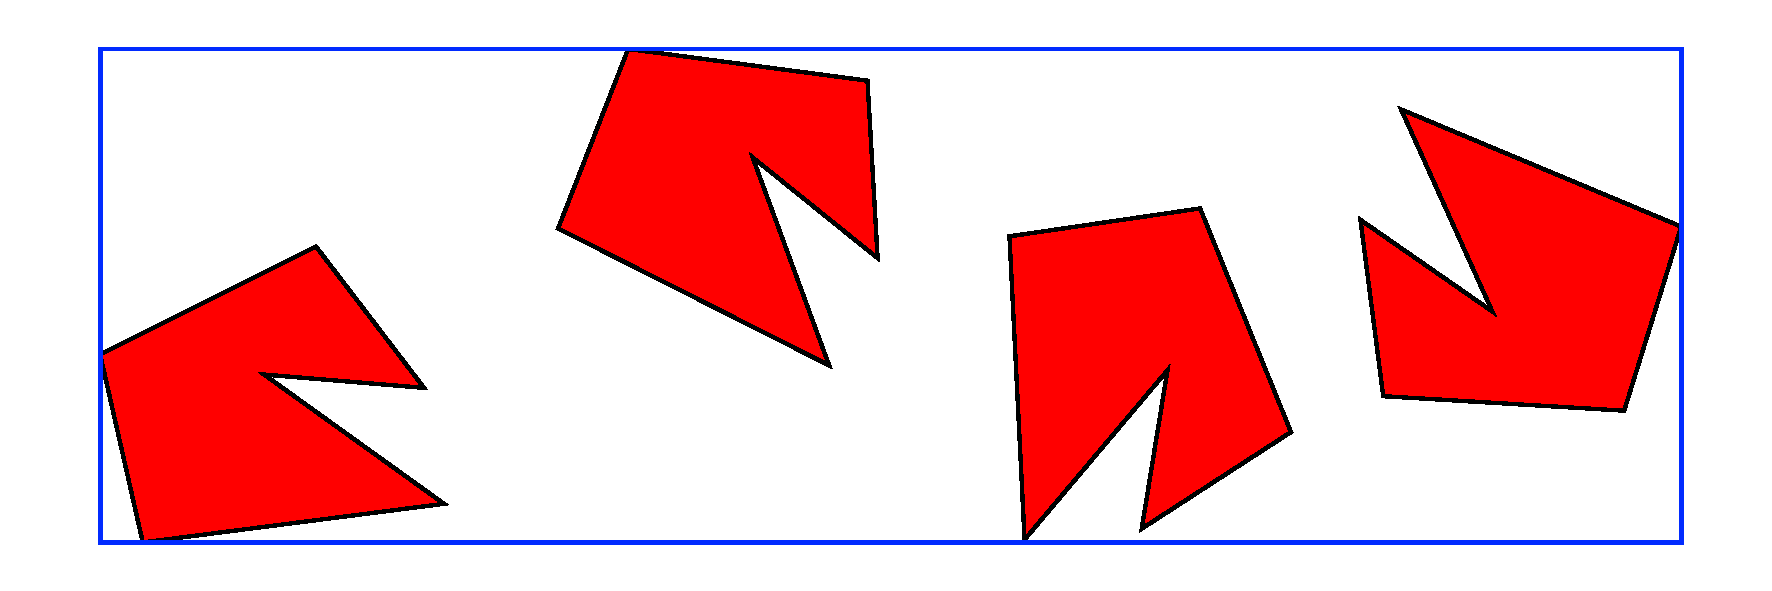
\includegraphics[width=0.75\textwidth]{images/tgeometryi_bbox.pdf}
    \caption{Bounding box of a tgeometryi}
    \label{fig:tgeometryi_bbox}
\end{figure}


The last case that needs to be handled is the computation of the bounding box of a moving region of sequence duration. Applying the same method as for regions of instant set duration does not work anymore since the vertices of the regions do not move linearly when the region is rotating. This means that some vertices will go outside the smallest bounding box containing both the start and end regions. A trivial example is when a square rotates 90 degrees without translating. The bounding box containing its start and end vertices will just be the square itself, but the corners of the square exited this bounding box during the rotation. 

A more advanced example can be seen in Figure \ref{fig:naive_bbox_error}, where the bounding box is shown in blue, and the path traversed by the moving region is shown in green. We can see that the moving region goes outside this naively computed bounding box.

\begin{figure}[h!]
    \centering
    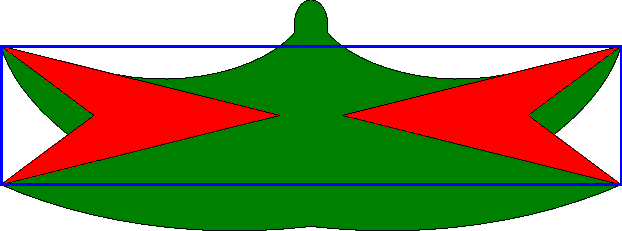
\includegraphics[width=0.75\textwidth]{images/naive_bbox_error.pdf}
    \caption{Error when computing the bounding box of a \lstinline+tgeometryseq+}
    \label{fig:naive_bbox_error}
\end{figure}

To solve this issue, we imagined two possible alternatives. First of all, if the traversed area (see Section \ref{section:traversed_area}) of the temporal region is known, we can just take the bounding box of this area, which will be indeed the minimal bounding box containing the moving region completely. However, since computing this traversed area is a computationally heavy operation, we propose another method that computed a bounding box more efficiently. This solution produces a correct but non-optimal bounding box. The bounding box is correct because the region will never exit this box during its movement, but non-optimal. Indeed, it will usually not be the smallest bounding box that can be found. These assumptions are still sufficient for the bounding box to be used for multiple purposes, so this solution has been implemented in MobilityDB.

To compute this bounding box for sequences, a similar procedure as for instance sets is used. The only difference is that when computing the bounding boxes of the instants, a \textit{rotating bounding box} algorithm is used instead of the PostGIS bounding box functions. This rotating bounding box algorithm works as follows:

\begin{enumerate}
    \item Find the vertex furthest from the rotation centre. In our case, the rotation centre is the centroid of the polygon representing the region. This step can be done with a linear search through the vertices.
    \item Compute the distance $d_{max}$ between the rotation centre and this vertex.
    \item Create a square of side $2*d_{max}$, centred around the rotation centre.
    \item Return this square as the rotating bounding box.
    \item (optional) Also return $d_{max}$ to be used for the following instants, since this value does not change if the region and the rotation centre of the region stay the same. If this is done, we can skip step 1 and 2 when computing the next rotating bounding boxes.
\end{enumerate}

\begin{figure}[h!]
    \centering
    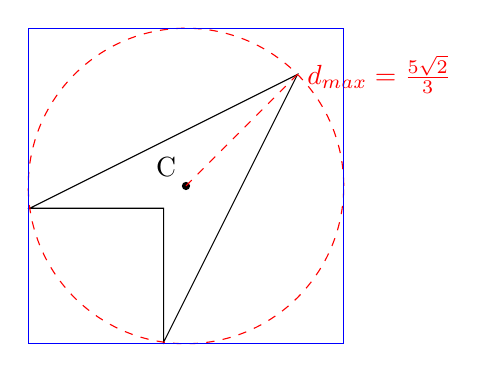
\begin{tikzpicture}[scale=0.85]
        \draw (-1, 1) -- (1, 1) -- (1, -1) -- (3, 3) -- cycle;
        \filldraw (4/3, 4/3) circle[radius=1.5 pt] node[anchor=south east] {C};
        \draw[red, dashed] (4/3, 4/3) -- (3, 3) node[anchor=west] {$d_{max} = \frac{5\sqrt{2}}{3}$};
        \draw[red, dashed] (4/3, 4/3) circle (2.357);
        \draw[blue] (4/3 - 2.357, 4/3 - 2.357) -- (4/3 - 2.357, 4/3 + 2.357) -- (4/3 + 2.357, 4/3 + 2.357) -- (4/3 + 2.357, 4/3 - 2.357) --cycle;
    \end{tikzpicture}
    \caption{Rotating bounding box around a region}
    \label{fig:rotating_bbox}
\end{figure}

This algorithm will return a bounding box which completely contains the given region, independently of any rotation applied to it around its rotation centre. After computing the bounding boxes of all the instants, the resulting bounding box will simply be the smallest box containing all the bounding boxes of the instants. Depending on the temporal geometry, this bounding box will be close or far from the optimal bounding box. If the polygon representing the region is relatively 'round', and the region rotates quickly, this bounding box will be quite accurate. If, however, the region is long but thin and does not rotate a lot, the bounding box will be much bigger than the optimal bounding box.

For this reason, this solution for bounding boxes might not be usable for some functions requiring an optimal (or almost optimal) bounding box and has to be handled carefully. It does, however, serve its purpose when it is used to prune the input set of some functions. For example, when we want to compute all temporal regions which are closer than a certain distance $d$ from each other at some instant during their movement, these sub-optimal bounding boxes can still be used but will simply prune a smaller set than if the boxes were optimal.

\subsection{Normalization}
\label{section:normalization}

When comparing moving objects, it is important to have identical objects being represented in the same way to allow for an efficient comparison process. This will be done by applying a normalization process on the given moving objects. Every sequence or sequence set that represents the same moving object will thus have the same internal representation after normalization. This normalization process is applied when creating a new moving object from an input or when merging multiple objects (for example, when combining two sequences of the same region). During normalization, redundant instants that could be recomputed by interpolating between two other instants are removed. For instants and instant sets, there is no normalization process, since we do not assume any interpolation process between instants, and thus we cannot have redundant instants. A simple example of a moving point is shown below to visualize the concept of normalization.

\begin{figure}[h!]
\centering
\vspace{.5 cm}
\begin{subfigure}[b]{0.475\textwidth}
    \centering
    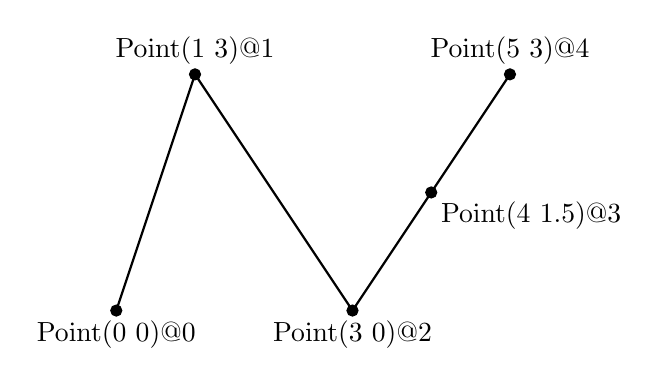
\begin{tikzpicture}
    \draw[thick] (0, 0) -- (1, 3) -- (3, 0) -- (5, 3);
    \filldraw[black] (0, 0) circle (2pt) node[anchor=north] {\lstinline{Point(0 0)@0}};
    \filldraw[black] (1, 3) circle (2pt) node[anchor=south] {\lstinline{Point(1 3)@1}};
    \filldraw[black] (3, 0) circle (2pt) node[anchor=north] {\lstinline{Point(3 0)@2}};
    \filldraw[black] (4, 1.5) circle (2pt) node[anchor=north west] {\lstinline{Point(4 1.5)@3}};
    \filldraw[black] (5, 3) circle (2pt) node[anchor=south] {\lstinline{Point(5 3)@4}};
    \end{tikzpicture}
    \caption{Before normalization}
\end{subfigure}
\hfill
\begin{subfigure}[b]{0.475\textwidth}
    \centering
    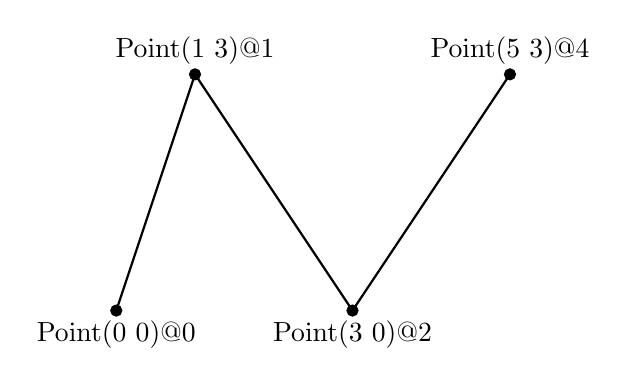
\begin{tikzpicture}
    \draw[thick] (0, 0) -- (1, 3) -- (3, 0) -- (5, 3);
    \filldraw[black] (0, 0) circle (2pt) node[anchor=north] {\lstinline{Point(0 0)@0}};
    \filldraw[black] (1, 3) circle (2pt) node[anchor=south] {\lstinline{Point(1 3)@1}};
    \filldraw[black] (3, 0) circle (2pt) node[anchor=north] {\lstinline{Point(3 0)@2}};
    \filldraw[black] (5, 3) circle (2pt) node[anchor=south] {\lstinline{Point(5 3)@4}};
    \end{tikzpicture}
    \caption{After normalization}
\end{subfigure}
\caption{Normalization of a temporal point}
\label{fig:tgeopointseq_normalization}
\end{figure}

Normalizing the representation of moving objects is important in multiple aspects. First, removing redundant instants in sequences and sequence sets makes the stored objects smaller. Secondly, having a unique representation for every moving object also allows to compare them for equality much more easily than if multiple representations of the same moving object are allowed.

As said previously, normalizing happens only in sequences and sequence sets. Normalization in sequence set can be seen as joining two sequences when the last instant of the first sequence is identical to the first instant of the second one and then normalizing the resulting sequence. In the following discussion, we will thus only focus on normalizing a single sequence.

To explain the normalization process of a moving region of sequence duration, we will first describe the normalization process of a moving point of sequence duration, since both processes are analogous. The interpolation technique used for moving points is a simple linear interpolation. In a sequence of points defined at increasing time instants, when three subsequent points are collinear and the ratio of their distance in the time dimension is the same as the ratio of their distance in 2d (or 3d) space, then the middle point is considered redundant since it could easily be recomputed using interpolation. This situation can be seen in Figure \ref{fig:tgeopointseq_normalization}.

Normalizing a moving region is done similarly. The main difference here is that we do not check for collinearity of points, but we check for collinearity of transformation vectors (\lstinline+rtransform+ values). Three transformation vectors are collinear if their translation vectors are collinear in 2d space, and their rotation angles are also collinear with the same ratio as the translation vectors. To check collinearity of the rotation angles we have to handle edge cases since the angles are always between $-\pi$ and $\pi$. An example of collinear regions can be seen in Figure \ref{fig:collinear_regions}.

\begin{figure}[h!]
    \centering
    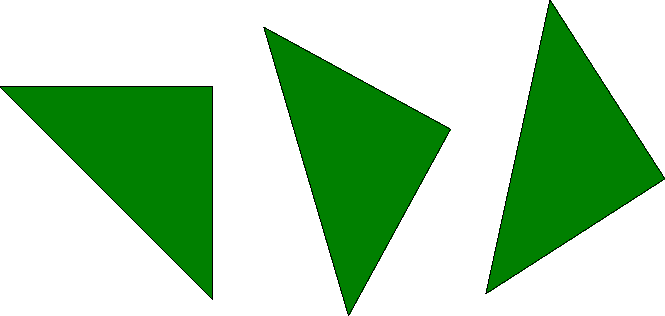
\includegraphics[width=0.6\textwidth]{images/collinear_regions.pdf}
    \caption[Example of collinear regions]{Example of collinear regions. The region is moving from left to right, and the corresponding rtransform values are: \lstinline{Rtransform(0, 0, 0), Rtransform(2, 0, -0.5), Rtransform(4, 0, -1)}. If the time difference between two subsequent instants is constant, then the regions are indeed collinear.}
    \label{fig:collinear_regions}
\end{figure}

When handling moving points, collinear points are considered redundant, since they can always be retrieved using interpolation. On the other hand, when handling moving regions, all collinear regions are not necessarily redundant. Indeed, since the interpolation method always interpolates two regions using the smallest angle between them, removing a collinear region could cause the interpolation to have a different direction of rotation than expected. This issue can be seen in Figure \ref{fig:collinear_not_redundant}.

\begin{figure}[h!]
    \centering
    \begin{subfigure}{.475\textwidth}
        \centering
        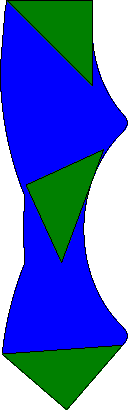
\includegraphics[width=0.2\textwidth]{images/collinear_not_redundant.pdf}
        \caption{Path taken with the collinear region (counter clockwise rotation)}
    \end{subfigure}
    \hfill
    \begin{subfigure}{.475\textwidth}
        \centering
        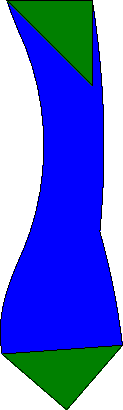
\includegraphics[width=0.2\textwidth]{images/collinear_not_redundant_2.pdf}
        \caption{Path taken without the collinear region (clockwise rotation)}
    \end{subfigure}
    \caption{Example of a collinear but not redundant instant in a moving region}
    \label{fig:collinear_not_redundant}
\end{figure}

This issue only comes up when the sum of the angles between three subsequent transformation vectors is larger than $\pi$. If this sum of angles is smaller than $\pi$, the collinear region is redundant and can be recomputed using interpolation. In this case, the region can simply be removed. However, if this is not the case, then the collinear region is not completely redundant since it gives information about the direction of rotation that would not be present if the region was simply removed. Leaving the region present is also not a possibility since this could result in multiple moving regions being identical while having a different representation.

\begin{figure}[h!]
    \centering
    \begin{subfigure}{.475\textwidth}
        \centering
        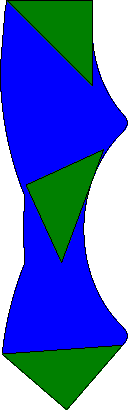
\includegraphics[width=0.2\textwidth]{images/collinear_not_redundant.pdf}
        \caption{First representation of the moving region}
    \end{subfigure}
    \hfill
    \begin{subfigure}{.475\textwidth}
        \centering
        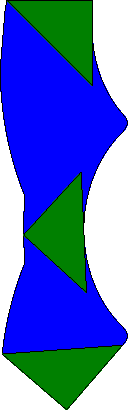
\includegraphics[width=0.2\textwidth]{images/same_tgeometry_diff_repr.pdf}
        \caption{Second representation of the same moving region}
    \end{subfigure}
    \caption[Two different representations of the same moving region]{Two different representations of the same moving region. In the second representation, the second instant is defined slightly later than in the first representation.}
    \label{fig:same_tgeometry_diff_repr}
\end{figure}

To solve this issue multiple ideas are possible. A first idea is to add the direction of rotation in the transformation vector. Since the interpolation of regions is done between two adjacent instants, this extra value would be defined with respect to the previous instant in the sequence. This contradicts with the other values in the stored transformation vector since previously the transformation vectors were defined with respect to the initial (first) region. This solution is thus feasible, but the values need to be handled with care.

Another solution is to add a \textit{dummy} region that would be the same for all objects representing the same moving region. This dummy region would serve as a kind of guide for the interpolation to preserve the correct direction of rotation. Although this technique would not always reduce the storage space, it does take care of the unique representation of the moving regions, which is the main concern. It is, however, possible that in some cases a dummy region can take the place of two regions instead of just one, and thus still reduce slightly the storage space.

This dummy region has to be well-defined so that every possible input representing the same moving region could be transformed into a unique representation. The definition should also try to minimize the number of dummy regions needed in this unique representation. We chose to define the dummy region in the following way: When three collinear regions have a combined angle of larger than $\pi$, the middle region will be replaced by a region which has a rotation of $\pi$ with respect to the first region if the rotation is counter-clockwise, or a rotation of $\pi - \epsilon$ with respect to the first region if the rotation is clockwise. The value of $\epsilon$ will be the same for all objects and has to be chosen so that the direction of rotation stay correct regardless of any rounding errors, while also being as small as possible. In practice, this value was chosen to be $\epsilon = 1\mathrm{e}{-5}$.

This definition produces a minimal amount of dummy regions, while still being able to recreate the initial movement of the region correctly. This method also produces unique representations and is thus a good way to normalize moving regions. This is the solution that has been chosen to implement in MobilityDB.

Theoretically, since the transformation that is stored for this dummy region is partially redundant, we could replace it with a single value representing the direction of rotation, or the intermediate angle. This is in principle feasible to reduce storage space even more, but that would mean that we need to handle a third type of object, which is not the best idea when we want to implement clean code. 

In practice, detecting if an instant is redundant or should be replaced by a dummy instant is done using the \lstinline{interpolate} and \lstinline{interpolate_long} functions described in Section \ref{section:utility_rtransform}. If the current instant can be computed with the \lstinline{interpolate} function using the previous an next instants as input, then the instant is redundant and can be removed. However, if the instant can be computed with the \lstinline{interpolate_long} function instead of \lstinline{interpolate}, then it means that the instant has to be replaced by a dummy instant.

\subsection{Standalone Instant}
\label{section:standalone_inst}

One particularity with temporal regions compared to all other types in MobilityDB is that some stored instants are not saved using the same  schema depending on where they occur in the temporal value. For example, a \lstinline{tgeometryinst} is stored as a pair of a polygon value and a timestamp. When an array of instants is given to the constructor \lstinline{tgeometryi}, every instant except the first is transformed into an instant with an \lstinline{rtransform} value. This means that to recompute one given instant, both this \lstinline+rtransform+ instant and the reference/initial instant (the first instant of the set) are needed, but the \lstinline+rtransform+ instant alone is not enough. 

This is different from all other temporal types, where all the instants are stored as they are received and can be retrieved without any post-processing. In MobiliyDB, since the structure of all temporal types is identical, multiple functions can manipulate all temporal types without needing to know exactly what the base type of the object is. For example, the \lstinline{instantN} function described in Section \ref{section:accessors} simply needs to retrieve the correct instant in the list, and return it. This is done using a function called \lstinline{temporali_inst_n} for instance sets and \lstinline{temporalseq_inst_n} for sequences. The returned instant can then be used as-is since it corresponds to a valid temporal instant.

When retrieving instants from a temporal region of instant set or sequence duration using the same functions, the returned instant cannot be used as is, since it does not represent a valid temporal region of instant duration (except if it is the first of the set). Instead, it needs to be combined with the region stored in the very first instant of the set. Sometimes retrieving a temporal instant with an \lstinline+rtransform+ value is what is needed, which is usually the case in region-specific functions, but in the most general functions (such as \lstinline{instantN} used as an example before) this is not the case, and a \textit{standalone} instant is required for the function to work.

To solve this issue, the new functions \lstinline{temporali_standalone_inst_n} for instant sets and \lstinline{temporalseq_standalone_inst_n} for sequences have been added, which returns a valid temporal instant. One thing to note is that the two initial functions only returned a pointer to the correct instant in the list since a copy is not necessarily needed. The new functions do the same, except when returning a \lstinline+tgeometryinst+ that was recomputed from an \lstinline+rtransform+ and a region instant. In this case, the returned instant is a newly created one, whose memory has to be correctly freed after it is used.

One might think that the same strategy has to be applied when retrieving a sequence from a temporal sequence set, but this is not the case. Indeed, as explained in Section \ref{section:internal_repr_s}, all sequences in the set are stored using the same schema, so as long as the first sequence can be handled correctly, which is the case with the \lstinline{temporalseq_standalone_inst_n}, all subsequent sequences can be manipulated similarly.

However, if the solution chosen in Section \ref{section:internal_repr_s} was the second one, where subsequent sequences are also preprocessed to only contain \lstinline+rtransform+ values and take up less storage space, then this would not be the case anymore, and a new function that can return a standalone sequence would also be needed.

\subsection{Traversed Area}
\label{section:traversed_area}

One function which is not yet explained but which is relatively important when handling moving regions is the computation of the \textit{traversed area}. By traversed area, we mean the set of all points that were touched by or contained in the region at some point during its movement. This is analogous in its uses to computing the trajectory of moving points but is quite a bit harder to compute in practice since the edges of a traversed area are in general not straight edges because the region can rotate. Examples of the traversed area of multiple moving regions can be seen in Figure \ref{fig:traversed_area_examples}.

\begin{figure}[h!]
    \centering
    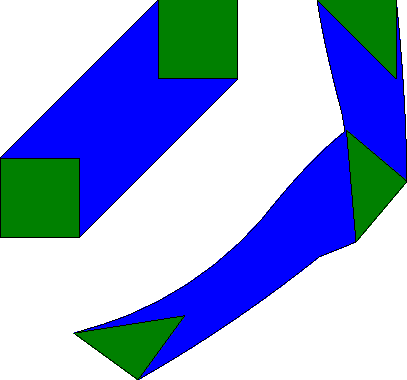
\includegraphics[width=0.4\textwidth]{images/traversed_area_example.pdf}
    \caption[Traversed area of two moving regions]{Traversed area (in blue) of two moving regions}
    \label{fig:traversed_area_examples}
\end{figure}

Having this traversed area precomputed for temporal regions simplifies the implementation of multiple functions. For example, computing the bounding box of a temporal sequence can be done by simply computing the bounding box of the traversed area of this sequence. Knowing if the temporal region will collide with a static point or region at some moment during its movement can also be done by simply checking if the traversed area intersects with the given point or region.

(Pre-)computing the traversed area for temporal regions is thus interesting, but how can it be done? The traversed area of a \lstinline+tgeometryinst+ is simply the region itself and is thus already stored as a polygon value in the instant. For temporal instant sets, since the region is only defined at specific moments, the traversed area will be the union of the regions of all instants, which can be stored as a PostGIS multipolygon. The same is true for temporal sequences with stepwise interpolation, and for temporal sequence set, the traversed area is the union of the traversed areas of all of its sequences. This leaves us with computing the traversed area of a \lstinline+tgeometryseq+.

An algorithm that can be used to compute the traversed area of a moving region is described in \cite{fmregion}, and the resulting area is stored in a newly defined type called \lstinline{cregion}, short for curved region, which can have three different types of segments: straight segments, trochoid segments and ravoid segments. The last two types are used to represent two different types of curves, \textit{trochoids} and \textit{ravoids}. A trochoid is used to represent the movement of a vertex of the region, and a ravoid is used to represent the movement of an edge of the region. These two types are described in \cite{fmregion}, and the functions used to describe them are also listed, but they are not added here since they will not effectively be used for our solution of the problem.

The solution given in the paper is also implemented in practice, and could thus be used by MobiltiyDB, but this would require us to define a new \lstinline{cregion} or \lstinline{cpolygon} type, and implement all of the needed geometric functions, such as \lstinline{inside}, \lstinline{overlap}, etc. However, one of the things that MobilityDB tries to do is to delegate geometric functions as much as possible to the existing PostGIS functions, since these are already implemented and optimized for the given types. To stay consistent with this idea, we thus want to store the traversed area in a PostGIS type, which enables us to use the PostGIS geometric functions without needing to re-implement them.

PostGIS has two different types that could be used to represent a traversed area: polygon and curvepolygon. If the moving region is not subject to any rotations, the resulting traversed area can be perfectly represented using a polygon, since there are no curves present. Otherwise, some parts of the area have to be represented using two different types of curves: trochoids and ravoids \cite{fmregion}. The curvepolygon, however, allows us to represent a circular curve, but neither trochoids nor ravoids. This means that no matter which polygon type is used, these curves will have to be approximated. Computing intersections between these two types of curves and straight segments is also computationally expensive, so instead of computing the traversed area as in \cite{fmregion} and then approximating it using a polygon or a curvepolygon, we will approximate the movement of the vertices and the edges of the region by straight segments, without ever using the trochoid or ravoid curve types. Since this solution uses only straight segments, the resulting traversed area can be stored in the polygon type. The current solution to this traversed area problem, together with remaining issues and possible improvements, is described below.

\subsubsection{Algorithm}

Given a \lstinline+tgeometryseq+ represented as $'[\mathcal{R}_0@t_0,\ \mathcal{T}_1@t_1,\ \mathcal{T}_2@t_2,\ ..., \ \mathcal{T}_{n-1}@t_{n-1}]'$, and assuming linear interpolation between the instants, we want to compute the area traversed by the region during its movement. The resulting area will be stored in a polygon object, which can in all generality contain holes, even if the base region does not contain any holes. Three different types of holes can be present in a traversed area, and these different types are shown in Figure \ref{fig:hole_types}. 

The first type is created from holes already present in the moving region (Figure \ref{fig:hole_type_1}). The second is created by a non-convex polygon in a single transformation, for example, when an L-shaped polygon rotates by $\pi$ and translates slightly (Figure \ref{fig:hole_type_2}). The last one can be created by any type of polygon and occurs when the moving region comes back at a previous position after multiple transformations (Figure \ref{fig:hole_type_3}).

The described algorithm computes a polygon without taking into account any holes in the traversed area. Using a slight modification of the algorithm, the third type of hole can be taken into account, but the two remaining types are not yet handled.

\begin{figure}[h!]
    \centering
    \begin{subfigure}{.3\textwidth}
        \centering
        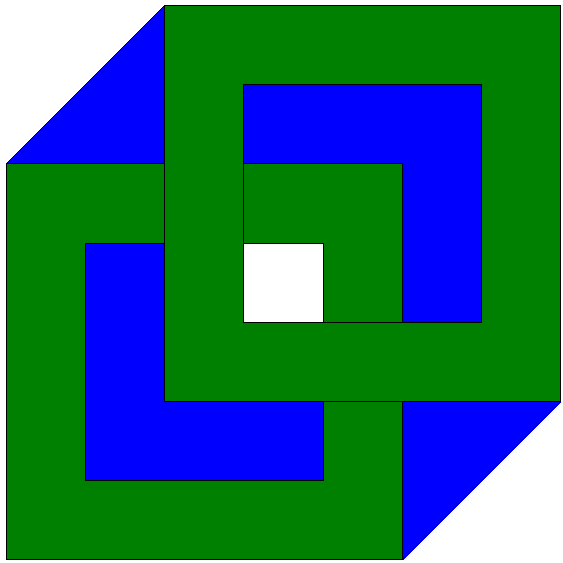
\includegraphics[width=\textwidth]{images/hole_1.pdf}
        \caption{Type 1}
        \label{fig:hole_type_1}
    \end{subfigure}
    \hfill
    \begin{subfigure}{.3\textwidth}
        \centering
        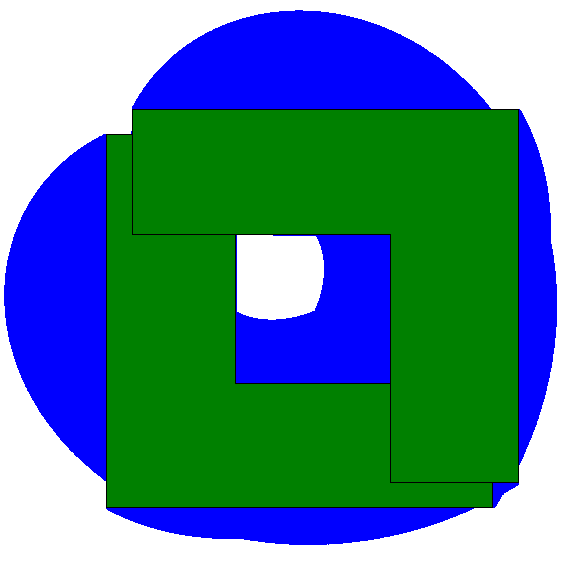
\includegraphics[width=\textwidth]{images/hole_2.pdf}
        \caption{Type 2}
        \label{fig:hole_type_2}
    \end{subfigure}
    \hfill
    \begin{subfigure}{.3\textwidth}
        \centering
        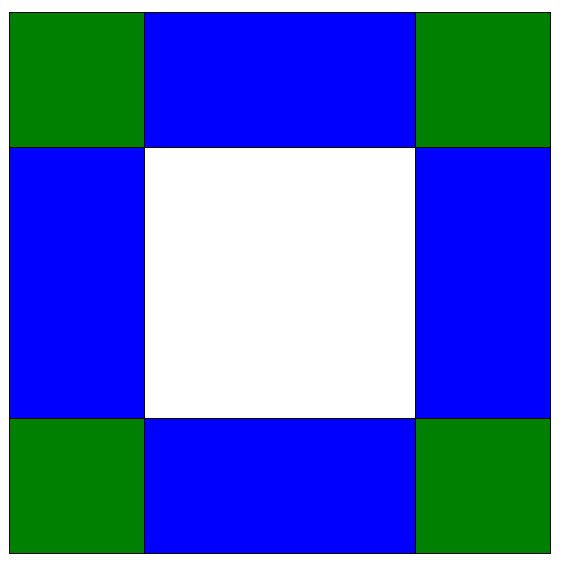
\includegraphics[width=\textwidth]{images/hole_3.pdf}
        \caption{Type 3}
        \label{fig:hole_type_3}
    \end{subfigure}
    \caption{Different types of holes created during the computation of the traversed area}
    \label{fig:hole_types}
\end{figure}

The algorithm works in three steps.

As a first step, we create a list of segments that will be used in the second step. This list of segments consists of both the edges of the polygons at different instants and segments created by the movement of the vertices of the polygons between these instants. We previously explained that we cannot use linear interpolation between the vertices to compute an interpolation between two instants since the movement of the vertices is not linear. This is only true for regions that rotate, so if the region is only translating, linear interpolation can be used as well. Since we want to represent the movement of the vertices of any moving region using straight segments, we will have to approximate this curve by a set of straight segments. 

To do this, we will assume that we can use linear interpolation between the vertices, and thus create a straight segment between these vertices to add to our list, for transformations which have a rotation which is smaller than a certain threshold ($\theta_{max}$) in absolute value. When the rotation $\theta$ is larger than this $\theta_{max}$, we will split the transformation into a set of $n$ transformations, with each transformation having the same rotation angle $\theta^*$. $n$ is chosen as the smallest integer value such that $\theta^* < \theta_{max}$.

\[
    n = \ceil*{\frac{\theta}{\theta_{max}}}
\]

The precision or correctness of the resulting traversed area depends entirely on the angle $\theta_{max}$, which has to be chosen small enough to keep the actual result sufficiently close from the desired result, but sufficiently large at the same time to not increase the computation time too much.

When receiving the temporal sequence as $'[\mathcal{R}_0@t_0,\ \mathcal{T}_1@t_1,\ \mathcal{T}_2@t_2,\ ...,\ \mathcal{T}_{n-1}@t_{n-1}]'$, we first add the needed amount of intermediate transformations to have the rotation between each subsequent transformation smaller than $\theta_{max}$. When this is done, the edges of the polygon defined by the first and last instant are put into a list. Then the segments created by the movement of the vertices during every transformation, as well as the segments corresponding to the edges of the polygon after each transformation, are also added to the list.

The second step transforms this list of segments into a planar graph by considering the endpoints of the segments, as well as intersections of segments, as vertices of the graph. This is internally stored as a mapping of vertices to a list of neighbour vertices. Doing this essentially consists of computing all the intersections in the received list of segments, and then computing for all vertices and intersections the list of neighbours. Two points are neighbours if there exists a segment containing both points, and no other vertex or intersection is present between them on that same segment. A visual representation of this planar graph can be seen in Figure \ref{fig:planar_graph}.

Computing all intersections of the set of segments is currently done naively (by testing all pairs of segments), but this could be improved by implementing the \textit{Bentley–Ottmann algorithm} \cite{computational_geometry}, which is a sweep-line algorithm with smaller time complexity than the naive solution when the number of intersections is not too large.

Lastly, the traversed area is computed from this planar graph. This is done by starting at the left-most vertex of the graph, and iteratively computing the next vertex of the traversed area until the start point is reached again. Computing the next vertex is done by taking the first neighbour of the current vertex when listing them in counterclockwise order starting from the previous vertex (which is one of the neighbours of the current vertex). By storing every vertex encountered in a list and stopping when the start vertex is reached, we obtain the polygon representing the traversed area of the moving region.

\begin{figure}[h!]
    \centering
    \begin{subfigure}{.3\textwidth}
        \centering
        
\includegraphics[width=0.8\textwidth]{images/process_regions.pdf}
        \caption{Instants defining the moving regions}
    \end{subfigure}
    \hfill
    \begin{subfigure}{.3\textwidth}
        \centering
        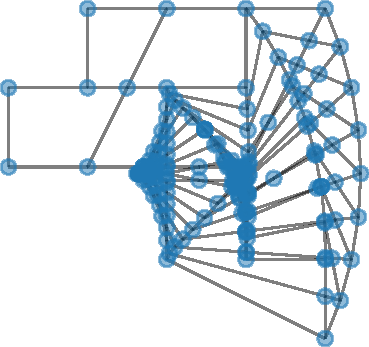
\includegraphics[width=0.8\textwidth]{images/process_planar_graph.pdf}
        \caption{Planar graph created from the computed segments}
        \label{fig:planar_graph}
    \end{subfigure}
    \hfill
    \begin{subfigure}{.3\textwidth}
        \centering
        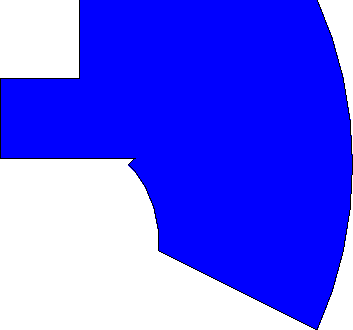
\includegraphics[width=0.8\textwidth]{images/process_traversed_area.pdf}
        \caption{Resulting traversed area}{}
    \end{subfigure}
    \caption[Process of computing the traversed area of a moving region]{Process of computing the traversed area of a moving region starting from a sequence of instants.}
    \label{fig:traversed_area_process}
\end{figure}

As said previously, the polygon representing a traversed area can, in all generality, have an arbitrary amount of inner rings (holes in the area). However, the described algorithm does not compute these inner rings and instead returns a polygon without any holes. Figure \ref{fig:hole_types} shows three kinds of holes, that are created in three different ways. One of them is created when the moving region comes back to a previous position after a certain amount of subsequent transformations. For a hole like this to be present, the temporal sequence must have at least three instants, which means that the region is subject to at least two transformations.

Computing a traversed area containing this third kind of hole is possible by adapting the previous algorithm slightly. Instead of computing the traversed area of the complete sequence in one go, we compute the traversed area between each pair of subsequent instants and store each of them in a list. The complete traversed area will then simply be the region created by the union of all polygons in this list. Computing this can be done using the PostGIS \lstinline{ST_Union} function.